% !TEX encoding = UTF-8 Unicode

\documentclass[a4paper]{article}

\usepackage{color}
\usepackage{url}
\usepackage[T2A]{fontenc} % enable Cyrillic fonts
\usepackage[utf8]{inputenc} % make weird characters work
\usepackage{graphicx}

\usepackage[english,serbian]{babel}
%\usepackage[english,serbianc]{babel} %ukljuciti babel sa ovim opcijama, umesto gornjim, ukoliko se koristi cirilica

\usepackage[unicode]{hyperref}
\hypersetup{colorlinks,citecolor=green,filecolor=green,linkcolor=blue,urlcolor=blue}

\DeclareUnicodeCharacter{0301}{\'{e}}

%\newtheorem{primer}{Пример}[section] %ćirilični primer
\newtheorem{primer}{Primer}[section]

\title{Roboti kao nastavnici\small \\Seminarski rad u okviru kursa\\Tehničko i naučno pisanje\\Matematički fakultet}
\author{Jovan Mijajlović, jovan.mijajlovic03@gmail.com\\Miona Sretenović, sretenovicmiona7@gmail.com\\Mina Protić, minaproticc@gmail.com\\Mihailo Marković, mihailoo003@gmail.com}
\date{7. decembar 2022.}

\begin{document}
\maketitle

\abstract{
Tema ovog seminarskog rada su edukativni roboti i njihova primena u nastavi. Postavlja se glavno pitanje, da li roboti mogu da zamene ljude u nastavi? U nastavku rada potrudićemo se da odgovorimo na ova pitanje.
}

\tableofcontents
\newpage

\section{Uvod}
\label{sec:uvod}

U prvom pogljavlju govorićemo o inovacijama u obrazovanju i implementaciji tehnologije u nastavi. Zatim, u drugom ćemo pricati o nastavnicima, o njihovoj ulozi i njihovom uticaju na nastavu. Nakon toga ćemo u trećem pogljavlju pričati uopšteno o robotima kao i o njihovoj primeni na nastavu.

\section{Implementacija tehnologije u nastavi}
\label{sec:naslov1}

Razvoj tehnologije kao i razvoj računara i njihovih znanja poslednjih decenija veoma brzo je napredovao što je omogućilo veću primenu informacionih tehnologija, koje su dosta uticale na naš svakodnevni život. Zbog sve veće upotrebe digitalnih tehnologija u svakodnevnom životu javlja se sve veća potreba za digitalnim opismenjavanjem ljudi. Kako stariji tako i mladi danas moraju imati neko “osnovno” znanje kada je reč o informacionim tehnologijama. Danas je to neka vrsta pismenosti. Informacione tehnologije su postale deo naših života, navikli smo da koristimo računare, telefone, pametne satove, koji dosta olakšavaju naš život. Stoga potrebno je da svi znamo da ih koristimo. Na primer, danas nije potrebno ići do pošte ili banke, kako bismo platiti račune, već je sve moguće uraditi preko naših telefona ili računara. Takođe u školama se više ne koristi stari “tradicionalni” dnevnik, nego postoji elektronski dnevnik, kao i elektronski indeks na fakultetima.

Zaključujemo da informacione tehnologije nisu mogle da zaobiđu ni škole, vrtiće, fakultete. Sve možemo uraditi online, upis u školu, upis na fakultet... Za vreme pandemije korona virusa u skoro svim školama bila je uvedena onlajn nastava, koja predstavlja proces edukacije putem interneta. Tokom onlajn nastave koristili su se razni internet servisi, kao što su video pozivi, digitalni resursi, poput prezentacija, video snimaka, audio predavanja i pdf vodiča koje nam je omogućila najnovija tehnologija... (slika \ref{fig:online}) U skoro svim osnovnim školama informatika je postala obavezan predmet, na kome đaci od “malena” uče kako da koriste tehnologiju. U većini srednjih škola se uče razni programski jezici i programiranje. Svi uče i znaju kako da koriste osnovne servise, poput Microsoft Office paketa.

\begin{figure}[ht!]
\begin{center}
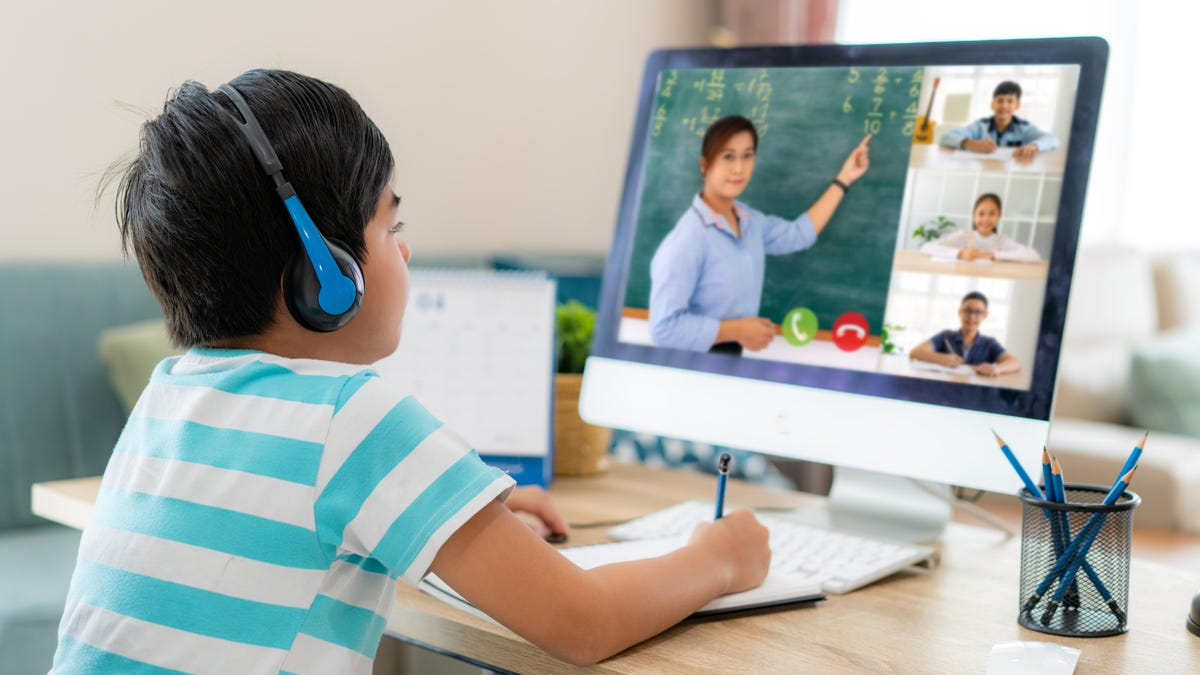
\includegraphics[scale=0.23]{online.jpg}
\end{center}
\caption{Onlajn nastava}
\label{fig:online}
\end{figure}
\end{document}